\documentclass[xetex,mathserif,serif]{beamer}
\usepackage{polyglossia}
\setdefaultlanguage[babelshorthands=true]{russian}
\usepackage{minted}
\usepackage{tabu}

\useoutertheme{infolines}

\usepackage{fontspec}
\setmainfont{FreeSans}
\newfontfamily{\russianfonttt}{FreeSans}

\setbeamertemplate{blocks}[rounded][shadow=false]
\setbeamercolor*{block title example}{fg=green!50!black,bg=green!20}
\setbeamercolor*{block body example}{fg=black,bg=green!10}

\setbeamercolor*{block title alerted}{fg=red!50!black,bg=red!20}
\setbeamercolor*{block body alerted}{fg=black,bg=red!10}

\tabulinesep=0.7mm

\title{Обзор библиотеки Guava}
\author[Юрий Литвинов]{Юрий Литвинов \newline \textcolor{gray}{\small\texttt{yurii.litvinov@gmail.com}}}

\date{17.04.2019г}

\begin{document}
	
	\frame{\titlepage}
	
	\section{Введение}

	\begin{frame}
		\frametitle{Guava}
		\textbf{Guava}\footnote{https://github.com/google/guava/wiki} --- одна из самых известных библиотек для Java
		\begin{itemize}
			\item Общего назначения
			\begin{itemize}
				\item Делает программирование на Java приятнее в мелочах
			\end{itemize}
			\item Новые коллекции, утилиты для ввода-вывода и многопоточности, хеширования, работы со строками и т.д. и т.п.
			\item Идеологически несколько отличается от JDK
			\begin{itemize}
				\item Не гарантирует обратную совместимость
				\item Не любит null
			\end{itemize}
		\end{itemize}
	\end{frame}

	\section{Утилиты}

	\begin{frame}[fragile]
		\frametitle{Preconditions}
		\textbf{Preconditions} --- что-то вроде продвинутого assert
		
		Пример:
		\begin{minted}{java}
checkArgument(i >= 0, "Argument was %s but expected nonnegative", i);
checkArgument(i < j, "Expected i < j, but %s > %s", i, j);
		\end{minted}
		Вместо
		\begin{minted}{java}
if (i >= 0) { 
    throw new IllegalArgimentException(
            "Argument was " + i + " but expected nonnegative");
}
		\end{minted}
\end{frame}

	\begin{frame}
		\frametitle{Что ещё бывает}
		\begin{scriptsize}
			\begin{tabu} {| X[0.9 l p] | X[1 l p] | X[1 l p] |}
				\tabucline-
				Сигнатура                                          & Описание                                                                                            & Бросаемое исключение      \\
				\tabucline-
				\everyrow{\tabucline-}
				checkArgument(boolean)                             & Проверить условие на аргумент                                                                       & IllegalArgumentException  \\
				checkNotNull(T)                                    & Проверить на не $null$                                                                              & NullPointerException      \\
				checkState(boolean)                                & Проверить состояние объекта безотносительно параметров (например, состояние итератора)              & IllegalStateException     \\
				checkElementIndex(int index, int size)             & Проверить, что $index$ от $0$ до $size - 1$                                                         & IndexOutOfBoundsException \\
				checkPositionIndex(int index, int size)            & Проверить, что $index$ от $0$ до $size$                                                             & IndexOutOfBoundsException \\
				checkPositionIndexes(int start, int end, int size) & Проверить, что переданный полуинтервал является валидным подынтервалом для списка заданного размера & IndexOutOfBoundsException \\
			\end{tabu}
		\end{scriptsize}
	\end{frame}

	\begin{frame}[fragile]
		\frametitle{MoreObjects}
		\begin{minted}{java}
// Returns "ClassName{x=1}"
MoreObjects.toStringHelper(this)
    .add("x", 1)
    .toString();

// Returns "MyObject{x=1}"
MoreObjects.toStringHelper("MyObject")
    .add("x", 1)
    .toString();
		\end{minted}
\end{frame}

	\begin{frame}[fragile]
		\frametitle{ComparisonChain}
		Класс \textbf{ComparisonChain} нужен для быстрой реализации \mintinline{java}|compareTo()|. Пример:
		
		\begin{minted}{java}
   public int compareTo(Foo that) {
     return ComparisonChain.start()
         .compare(this.aString, that.aString)
         .compare(this.anInt, that.anInt)
         .compare(this.anEnum, that.anEnum, Ordering.natural().nullsLast())
         .result();
   }
		\end{minted}

		Класс \textbf{Ordering} нужен для быстрой реализации \mintinline{java}|Comparator|.
\end{frame}

	\begin{frame}[fragile]
		\frametitle{Throwables}
		\textbf{Throwables} делает работу с исключениями несколько более удобной. Пример:

		\begin{minted}{java}
   try {
     someMethodThatCouldThrowAnything();
   } catch (IKnowWhatToDoWithThisException e) {
     handle(e);
   } catch (Throwable t) {
     Throwables.propagateIfPossible(t, OtherException.class);
     throw new RuntimeException("unexpected", t);
   }
		\end{minted}

		\begin{scriptsize}
			Ещё есть \mintinline{java}|List<Throwable> getCausalChain(Throwable throwable)|, \mintinline{java}|Throwable getRootCause(Throwable throwable)|, \mintinline{java}|void throwIfInstanceOf(Throwable throwable, Class<X> declaredType)|
		\end{scriptsize}
\end{frame}

 	\section{Коллекции}

	\begin{frame}
		\frametitle{Немутабельные коллекции}
		Для каждой коллекции из стандартной библиотеки и каждой коллекции из Guava есть Immutable-вариант, например, \textbf{ImmutableMap}, \textbf{ImmutableList} и т.д. Зачем:
		\begin{itemize}
			\item многопоточность
			\item эффективность
			\item хороший стиль
		\end{itemize}
		\mintinline{java}|Collections.unmodifiable...| из JDK не совсем немутабельны. \textbf{Immutable*}-коллекция никогда не меняет своих элементов.
	\end{frame}

	\begin{frame}
		\frametitle{Как создать немутабельную коллекцию}
		\begin{itemize}
			\item \mintinline{java}|copyOf|, например, \mintinline{java}|ImmutableSet.copyOf(set)|
			\item \mintinline{java}|of|, например, \mintinline{java}|ImmutableSet.of("a", "b", "c")| или \mintinline{java}|ImmutableMap.of("a", 1, "b", 2)|
			\item метод \mintinline{java}|asList()| у немутабельных коллекций, который возвращает \mintinline{java}|ImmutableList|.
		\end{itemize}
		\mintinline{java}|copyOf| не копирует коллекцию, если это не приведёт к проблемам
	\end{frame}

	\begin{frame}
		\frametitle{Multiset}
		\textbf{Multiset} --- мутабельное мультимножество: неупорядоченный \mintinline{java}|ArrayList<E>| или \mintinline{java}|Map<E, Integer>|
		\vspace{5mm}

		\begin{scriptsize}
			\begin{tabu} {| X[0.4 l p] | X[1 l p] |}
				\tabucline-
				Метод            & Описание                                                                                          \\
				\tabucline-
				\everyrow{\tabucline-}
				count(E)         & Возвращает количество вхождений элемента                                                          \\
				elementSet()     & Возвращает множество (нормальное) различных элементов (на самом деле, view)                       \\
				entrySet()       & Возвращает множество объектов Multiset.Entry<E>, у которых можно узнать элемент и число вхождений \\
				add(E, int)      & Добавляет указанное количество вхождений указанного элемента                                      \\
				remove(E, int)   & Удаляет указанное количество вхождений указанного элемента                                        \\
				setCount(E, int) & Устанавливает количество вхождений заданного элемента в заданное число                            \\
				size()           & Возвращает общее количество элементов в мультимножестве                                           \\
			\end{tabu}
		\end{scriptsize}
	\end{frame}

	\begin{frame}
		\frametitle{Multiset}
		\textbf{Multiset} --- не просто Map:
		\begin{itemize}
			\item количество вхождений элемента не может быть отрицательным
			\item установление количества вхождений элемента в 0 равносильно удалению всех его вхождений
			\item \mintinline{java}|multiset.count(elem)| для элемента, не принадлежащего мультимножеству, вернёт 0
		\end{itemize}

		Реализации (примерно соответствуют стандартным реализациям Map): \textit{HashMultiset}, \textit{TreeMultiset}, \textit{LinkedHashMultiset}, \textit{ConcurrentHashMultiset}, \textit{ImmutableMultiset}
	\end{frame}

	\begin{frame}
		\frametitle{Multimap}
		\textbf{Multimap} --- можно понимать как Map с неуникальными ключами или как Map, отображающий ключ в список значений
		\begin{itemize}
			\item Первая интерпретация <<из коробки>>, вторая --- методом \mintinline{java}|asMap()|, который возвращает \mintinline{java}|Map<K, Collection<V>>|
			\item Ключ всегда отображается в хотя бы оно значение
			\item Интерфейсы-наследники \textbf{ListMultimap} и \textbf{SetMultimap}
		\end{itemize}

		Реализации: \textit{ArrayListMultimap}, \textit{HashMultimap}, \textit{LinkedListMultimap}, \textit{LinkedHashMultimap}, \textit{TreeMultimap}, \textit{ImmutableListMultimap}, \textit{ImmutableSetMultimap}
	\end{frame}

	\begin{frame}[fragile]
		\frametitle{Multimap, пример}
		\begin{minted}{java}
Set<Person> aliceChildren = childrenMultimap.get(alice);
aliceChildren.clear();
aliceChildren.add(bob);
aliceChildren.add(carol);
		\end{minted}
		Результат \mintinline{java}|get()| --- это вид на коллекцию, так что \mintinline{java}|childrenMultimap| тоже изменится. Кстати, \mintinline{java}|get(key)| всегда возвращает коллекцию, возможно, пустую.
\end{frame}

	\begin{frame}
		\frametitle{BiMap}
		\textbf{BiMap} --- отображает ключи в значения и обратно
		\begin{itemize}
			\item И ключи, и значения должны быть уникальны
			\item Затирать старое значение можно методом \mintinline{java}|BiMap.forcePut(key, value)|
			\item Метод \mintinline{java}|inverse()| возвращает обратный \mintinline{java}|BiMap|
		\end{itemize}

		Реализации: \textit{HashBiMap}, \textit{ImmutableBiMap}, \textit{EnumBiMap}, \textit{EnumHashBiMap}
	\end{frame}

	\begin{frame}[fragile]
		\frametitle{Table}
		\textbf{Table} --- двумерная таблица, \mintinline{java}|Map<R, Map<C, V>>|
		
		\begin{minted}{java}
Table<DateOfBirth, LastName, PersonalRecord> records 
        = HashBasedTable.create();
records.put(someBirthday, "Schmo", recordA);
records.put(someBirthday, "Doe", recordB);
records.put(otherBirthday, "Doe", recordC);

// Возвращает Map, отображающий "Schmo" в recordA, 
// "Doe" в recordB
records.row(someBirthday); 
// Возвращает Map, отображающий someBirthday в recordB, 
// otherBirthday в recordC
records.column("Doe"); 
		\end{minted}
		
		Реализации: \textit{HashBasedTable}, \textit{TreeBasedTable}, \textit{ImmutableTable}, \textit{ArrayTable}
\end{frame}

	\begin{frame}[fragile]
		\frametitle{ClassToInstanceMap}
		\textbf{ClassToInstanceMap} --- отображение из класса в объект (\mintinline{java}|Map<Class<? extends B>, B>|)

		\begin{minted}{java}
ClassToInstanceMap<Number> numberDefaults 
        = MutableClassToInstanceMap.create();
numberDefaults.putInstance(Integer.class, Integer.valueOf(0));
		\end{minted}

		Реализации: \textit{MutableClassToInstanceMap} и \textit{ImmutableClassToInstanceMap}
\end{frame}

	\begin{frame}[fragile]
		\frametitle{RangeSet}
		\textbf{RangeSet} --- это набор промежутков: отрезков, интервалов или полуинтервалов:
		
		\begin{minted}{java}
RangeSet<Integer> rangeSet = TreeRangeSet.create();
rangeSet.add(Range.closed(1, 10));  // {[1, 10]}
rangeSet.add(Range.closedOpen(11, 15));  // {[1, 10], [11, 15)}
rangeSet.add(Range.closedOpen(15, 20));  // {[1, 10], [11, 20)}
rangeSet.add(Range.openClosed(0, 0));  // {[1, 10], [11, 20)}
rangeSet.remove(Range.open(5, 10));  // {[1, 5], [10, 10], [11, 20)}
		\end{minted}
		
		Умеет: автоматически объединять перекрывающие друг друга интервалы, делать дополнение к набору промежутков, пересечение с заданным промежутком, проверять на принадлежность точке набору промежутков, считать покрытие и т.д.
\end{frame}

	\begin{frame}[fragile]
		\frametitle{RangeMap}
		\textbf{RangeMap} отображает промежутки в некоторые значения:
		
		\begin{minted}{java}
RangeMap<Integer, String> rangeMap = TreeRangeMap.create();
rangeMap.put(Range.closed(1, 10), "foo"); // {[1, 10] => "foo"}

// {[1, 3] => "foo", (3, 6) => "bar", [6, 10] => "foo"}
rangeMap.put(Range.open(3, 6), "bar"); 
		\end{minted}
\end{frame}

	\begin{frame}
		\frametitle{Классы-утилиты}
		Для всех новых коллекций и многих коллекций из JDK есть классы-утилиты (для \textit{Multiset} есть класс \textit{Multisets}, для \textit{Table} --- \textit{Tables}, для \textit{List} --- \textit{Lists} и т.д.)
		\begin{itemize}
			\item Не так полезны с выходом Java 8
			\item В отличие от JDK, в основном ленивы
			\item Могут быть короче и аккуратнее, чем стандартные
		\end{itemize}
	\end{frame}

	\begin{frame}[fragile]
		\frametitle{Классы-утилиты, пример 1}
		\begin{minted}{java}
Set<String> wordsWithPrimeLength 
        = ImmutableSet.of("one", "two", "three"
                         , "six", "seven", "eight");
Set<String> primes = ImmutableSet.of(
        "two", "three", "five", "seven");

SetView<String> intersection 
        = Sets.intersection(primes, wordsWithPrimeLength);
return intersection.immutableCopy();
		\end{minted}
\end{frame}

	\begin{frame}[fragile]
		\frametitle{Классы-утилиты, пример 2}
		\begin{minted}{java}
Set<String> animals = ImmutableSet.of("gerbil", "hamster");
Set<String> fruits = ImmutableSet.of("apple", "orange", "banana");

Set<List<String>> product = Sets.cartesianProduct(animals, fruits);
// {{"gerbil", "apple"}, {"gerbil", "orange"}, {"gerbil", "banana"},
//  {"hamster", "apple"}, {"hamster", "orange"}, {"hamster", "banana"}}

Set<Set<String>> animalSets = Sets.powerSet(animals);
// {{}, {"gerbil"}, {"hamster"}, {"gerbil", "hamster"}}
		\end{minted}
\end{frame}

	\begin{frame}[fragile]
		\frametitle{Классы-утилиты, пример 3}
		\begin{minted}{java}
Map<String, Integer> left = ImmutableMap.of("a", 1, "b", 2, "c", 3);
Map<String, Integer> right = ImmutableMap.of("b", 2, "c", 4, "d", 5);
MapDifference<String, Integer> diff = Maps.difference(left, right);

diff.entriesInCommon();  // {"b" => 2}
diff.entriesDiffering();  // {"c" => (3, 4)}
diff.entriesOnlyOnLeft();  // {"a" => 1}
diff.entriesOnlyOnRight();  // {"d" => 5}
		\end{minted}
\end{frame}

	\begin{frame}
		\frametitle{Средства быстрого создания коллекций}
		\textbf{Forwarding Decorators} --- заготовки для реализации стандартных интерфейсов, как \textbf{Abstract*} из JDK
		\begin{itemize}
			\item Вместо наследования используется композиция
			\item Наследуемся от Forwarding Decorator-а из Guava, переопределяем метод \mintinline{java}|delegate()|
			\item \mintinline{java}|delegate()| должен возвращать <<декорируемую>> коллекцию, которой декоратор будет перенаправлять все непереопределённые запросы
			\item Позволяет динамически менять декорируемые объекты и даже выстраивать цепочки <<декораторов>>
		\end{itemize}
	\end{frame}

	\begin{frame}[fragile]
		\frametitle{Пример}
		\begin{minted}{java}
class AddLoggingList<E> extends ForwardingList<E> {
  final List<E> delegate; // декорируемый список
  @Override protected List<E> delegate() {
    return delegate;
  }
  @Override public void add(int index, E elem) {
    log(index, elem);
    super.add(index, elem);
  }
  @Override public boolean add(E elem) {
    return standardAdd(elem);  // реализуется в терминах add(int, E)
  }
  @Override public boolean addAll(Collection<? extends E> c) {
    return standardAddAll(c); // реализуется в терминах add
  }
}
		\end{minted}
\end{frame}

	\begin{frame}[fragile]
		\frametitle{Средства быстрого создания итераторов}
		\textbf{PeekingIterator} --- обёртка для итераторов, предоставлящая метод \mintinline{java}|peek()|. \textbf{AbstractIterator} и \textbf{AbstractSequentialIterator} позволяют быстро реализовать итератор:
		
		\begin{minted}{java}
Iterator<Integer> powersOfTwo 
        = new AbstractSequentialIterator<Integer>(1) {
    protected Integer computeNext(Integer previous) {
        return (previous == 1 << 30) ? null : previous * 2;
    }
};
		\end{minted}
\end{frame}

	\section{Графы}

	\begin{frame}
		\frametitle{Графы}
		Графы в Guava бывают трёх видов:
		\begin{itemize}
			\item \textbf{Graph} --- вершины и непомеченные рёбра
			\item \textbf{ValueGraph} --- наследник Graph, добавляющий метки на рёбрах
			\item \textbf{Network} --- граф, в котором и вершины, и рёбра имеют собственную идентичность
			\begin{itemize}
				\item outEdges(node)
				\item incidentNodes(edge)
				\item edgesConnecting(nodeU, nodeV)
				\item ...
				\item asGraph()
			\end{itemize}
		\end{itemize}
	\end{frame}

	\begin{frame}[fragile]
		\frametitle{Создание графов}
		Классы GraphBuilder, ValueGraphBuilder и NetworkBuilder (паттерн <<Строитель>>)
		\begin{minted}{java}
MutableGraph<Integer> graph = GraphBuilder.undirected().build();

MutableValueGraph<City, Distance> roads 
        = ValueGraphBuilder.directed().build();

MutableNetwork<Webpage, Link> webSnapshot 
        = NetworkBuilder.directed()
            .allowsParallelEdges(true)
            .nodeOrder(ElementOrder.natural())
            .expectedNodeCount(100000)
            .expectedEdgeCount(1000000)
            .build();
		\end{minted}
\end{frame}

	\begin{frame}
		\frametitle{Замечания}
		\begin{itemize}
			\item Почти все конкретные классы графов не экспортируются
			\item \textit{Graph}, \textit{ValueGraph} и \textit{Network} не предоставляют изменяющих граф методов, но есть их наследники \textit{MutableGraph}, \textit{MutableValueGraph} и \textit{MutableNetwork}
			\item \textit{ImmutableGraph}, \textit{ImmutableValueGraph} и \textit{ImmutableNetwork} гарантируют немутабельность графа
			\item Метод \mintinline{java}|copyOf()| выполняет мелкое (shallow) копирование
			\item Класс \textbf{Graphs} --- набор статических методов
			\begin{itemize}
				\item \mintinline{java}|hasCycle(Graph<?> graph)|
				\item \mintinline{java}|inducedSubgraph(Graph<N> graph, Iterable<? extends N> nodes)|
				\item \mintinline{java}|reachableNodes(Graph<N> graph, Object node)|
				\item \mintinline{java}|transitiveClosure(Graph<N> graph)|
			\end{itemize}
			\item Неплохо работает на графах порядка миллионов вершин
		\end{itemize}
	\end{frame}

	\begin{frame}[fragile]
		\frametitle{Пример 1}
		\begin{minted}{java}
MutableValueGraph<Integer, Double> weightedGraph 
    = ValueGraphBuilder.directed().build();

weightedGraph.addNode(1);
weightedGraph.putEdgeValue(2, 3, 1.5);  // добавляет 2 и 3
weightedGraph.putEdgeValue(3, 5, 1.5);  
...
weightedGraph.putEdgeValue(2, 3, 2.0);  // обновляет вес (2,3)
		\end{minted}
\end{frame}

	\begin{frame}[fragile]
		\frametitle{Пример 2}
		\begin{minted}{java}
MutableNetwork<Integer, String> network 
    = NetworkBuilder.directed().build();

network.addNode(1);
network.addEdge("2->3", 2, 3);  // добавляет 2 и 3

Set<Integer> successorsOfTwo = network.successors(2);
Set<String> outEdgesOfTwo = network.outEdges(2);

network.addEdge("2->3 too", 2, 3);  // исключение
network.addEdge("2->3", 2, 3);  // ничего не делает

Set<String> inEdgesOfFour = network.inEdges(4); // исключение
		\end{minted}
\end{frame}

	\section{Кеши}

	\begin{frame}[fragile]
		\frametitle{Пример работы с кешем}
		\begin{minted}{java}
LoadingCache<Key, Graph> graphs = CacheBuilder.newBuilder()
       .maximumSize(1000)
       .build(
           new CacheLoader<Key, Graph>() {
             public Graph load(Key key) throws AnyException {
               return createExpensiveGraph(key);
             }
           });

...
try {
    return graphs.get(key);
} catch (ExecutionException e) {
    throw new OtherException(e.getCause());
}
		\end{minted}
\end{frame}

	\begin{frame}[fragile]
		\frametitle{Вариант без CacheLoader-а}
		\begin{minted}{java}
Cache<Key, Value> cache = CacheBuilder.newBuilder()
    .maximumSize(1000)
    .build(); 
...
try {
    cache.get(key, () -> doThingsTheHardWay(key));
} catch (ExecutionException e) {
    throw new OtherException(e.getCause());
}
		\end{minted}
\end{frame}

	\begin{frame}
		\frametitle{Выталкивание значений из кеша}
		\begin{itemize}
			\item Чистка происходит только при записи и иногда при чтении
			\item \mintinline{java}|CacheBuilder.expireAfterAccess(long, TimeUnit)|
			\item \mintinline{java}|CacheBuilder.expireAfterWrite(long, TimeUnit)|
			\begin{itemize}
				\item \mintinline{java}|CacheBuilder.ticker(Ticker)|
			\end{itemize}
			\item \mintinline{java}|CacheBuilder.maximumWeight(long)| и интерфейс \mintinline{java}|Weigher|
			\item \mintinline{java}|Cache.invalidate(key)| и \mintinline{java}|Cache.invalidateAll()|
			\item Weak references
			\item \mintinline{java}|CacheBuilder.removalListener(RemovalListener)|
			\item \mintinline{java}|CacheBuilder.recordStats()| и \mintinline{java}|Cache.stats()|
		\end{itemize}
	\end{frame}

	\section{Функциональные идиомы}

	\begin{frame}
		\frametitle{Функциональные идиомы}
		С Java 8 не так актуально, но всё равно стоит посмотреть
		\begin{itemize}
			\item \mintinline{java}|Function<A, B>|
			\begin{itemize}
				\item \mintinline{java}|forMap(Map<A, B>)|, \mintinline{java}|compose(Function<B, C>, Function<A, B>)|, \mintinline{java}|constant(T)|, \mintinline{java}|identity()|
			\end{itemize}
			\item \mintinline{java}|Predicate<T>|
			\begin{itemize}
				\item \mintinline{java}|instanceOf(Class)|, \mintinline{java}|assignableFrom(Class)|, \mintinline{java}|contains(Pattern)|, \mintinline{java}|in(Collection)|, \mintinline{java}|isNull()|, \mintinline{java}|alwaysFalse()|, ...
			\end{itemize}
		\end{itemize}
	\end{frame}

	\section{Многопоточность}

	\begin{frame}
		\frametitle{ListenableFuture}
		\begin{itemize}
			\item \textbf{ListenableFuture} --- наследник обычного \textit{Future}, который добавляет метод \mintinline{java}|addListener(Runnable, Executor)|, что делает возможным много чего, например, связывать асинхронные операции в цепочки
			\item \textbf{FutureCallback<V>} --- позволяет подписаться на успешное и неудачное выполнение операции
			\item \textbf{Futures} 
			\begin{itemize}
				\item \mintinline{java}|addCallback(ListenableFuture<V>, FutureCallback<V>, Executor)|
				\item \mintinline{java}|transformAsync(ListenableFuture<A>,| \mintinline{java}|AsyncFunction<A, B>, Executor)|
				\item \mintinline{java}|allAsList(Iterable<ListenableFuture<V>>)|
				\item \mintinline{java}|successfulAsList(Iterable<ListenableFuture<V>>)|
			\end{itemize}
		\end{itemize}
	\end{frame}
	
	\begin{frame}[fragile]
		\frametitle{Пример}
		\begin{minted}{java}
ListeningExecutorService service 
        = MoreExecutors.listeningDecorator(
            Executors.newFixedThreadPool(10));
ListenableFuture<Explosion> explosion 
        = service.submit(() -> pushBigRedButton());
Futures.addCallback(explosion, new FutureCallback<Explosion>() {
  public void onSuccess(Explosion explosion) {
    walkAwayFrom(explosion);
  }
  public void onFailure(Throwable thrown) {
    battleArchNemesis();
  }
});
		\end{minted}
\end{frame}

	\begin{frame}
		\frametitle{Service}
		\textbf{Service} --- абстракция сервиса, который можно запустить и остановить, следит за своим состоянием
		\begin{itemize}
			\item \mintinline{java}|Service.State.NEW|
			\item \mintinline{java}|Service.State.STARTING|
			\item \mintinline{java}|Service.State.RUNNING|
			\item \mintinline{java}|Service.State.STOPPING|
			\item \mintinline{java}|Service.State.TERMINATED|
		\end{itemize}

		\textbf{ServiceManager} --- класс, управляющий несколькими сервисами (\mintinline{java}|startAsync()|, \mintinline{java}|stopAsync()|, \mintinline{java}|awaitHealthy()|, \mintinline{java}|awaitStopped()|, ...)
	\end{frame}

	\section{Утилиты работы со строками}

	\begin{frame}[fragile]
		\frametitle{Joiner и Splitter}
		Похожая функциональность есть в стандартной библиотеке, но классы из Guava немного удобнее
		\begin{itemize}
			\item Joiner
			
			\begin{minted}{java}
Joiner joiner = Joiner.on("; ").skipNulls();
return joiner.join("Harry", null, "Ron", "Hermione");
			\end{minted}
			\item Splitter

			\begin{minted}{java}
Splitter.on(',')
    .trimResults()
    .omitEmptyStrings()
    .split("foo,bar,,   qux");
			\end{minted}
		\end{itemize}
\end{frame}
	
	\begin{frame}[fragile]
		\frametitle{CharMatcher}
		\begin{minted}{java}
String noControl = CharMatcher.javaIsoControl().removeFrom(string);
String theDigits = CharMatcher.digit().retainFrom(string);
String spaced = CharMatcher.whitespace()
        .trimAndCollapseFrom(string, ' ');
String noDigits = CharMatcher.javaDigit().replaceFrom(string, "*");
String lowerAndDigit = CharMatcher
        .javaDigit()
        .or(CharMatcher.javaLowerCase())
        .retainFrom(string);
		\end{minted}
\end{frame}

	\begin{frame}[fragile]
		\frametitle{CaseFormat}
		\begin{minted}{java}
CaseFormat.UPPER_UNDERSCORE.to(
        CaseFormat.LOWER_CAMEL, "CONSTANT_NAME")); 
// "constantName"
		\end{minted}
		Умеет: 
		\begin{itemize}
			\item \mintinline{java}|LOWER_CAMEL| (lowerCamel)
			\item \mintinline{java}|LOWER_HYPHEN| (lower-hyphen)
			\item \mintinline{java}|LOWER_UNDERSCORE| (lower\_underscore)
			\item \mintinline{java}|UPPER_CAMEL| (UpperCamel)
			\item \mintinline{java}|UPPER_UNDERSCORE| (UPPER\_UNDERSCORE)
		\end{itemize}
\end{frame}

	\section{Event bus}

	\begin{frame}
		\frametitle{Event bus}
		\begin{itemize}
			\item Подсистема для связи компонентов программы так, чтобы им не надо было даже знать друг о друге
			\item Publisher-Subscriber
			\item Для замены Listener-ов из JDK
			\begin{itemize}
				\item Не предназначена для межпроцессного взаимодействия
				\item Не может сложную маршрутизацию, фильтры и т.д.
			\end{itemize}
			\item Использует аннотацию \mintinline{java}|@Subscribe| для методов-подписчиков
		\end{itemize}
	\end{frame}

	\begin{frame}[fragile]
		\frametitle{Пример}
		\begin{minted}{java}
class EventBusChangeRecorder {
  @Subscribe public void recordCustomerChange(ChangeEvent e) {
    recordChange(e.getChange());
  }
}
...
eventBus.register(new EventBusChangeRecorder());
...
public void changeCustomer() {
  ChangeEvent event = getChangeEvent();
  eventBus.post(event);
}
		\end{minted}
\end{frame}

	\section{Фильтр Блума}

	\begin{frame}
		\frametitle{Фильтр Блума}
		\begin{center}
			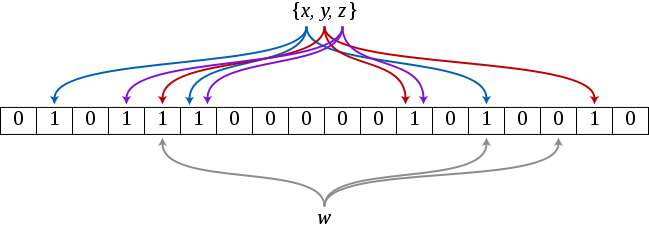
\includegraphics[width=0.9\textwidth]{bloomFilter.png}
		\end{center}

		Структура данных, умеющая очень эффективно определять, что элемента в множестве точно нет или с некоторой (задаваемой) вероятностью есть.
	\end{frame}

	\begin{frame}[fragile]
		\frametitle{Пример}
		\begin{minted}{java}
BloomFilter<Person> friends 
        = BloomFilter.create(personFunnel, 500, 0.01);
for(Person friend : friendsList) {
  friends.put(friend);
}
...
if (friends.mightContain(dude)) {
  // Вероятность того, что dude не друг, составляет здесь 1%
  ...
}
		\end{minted}
\end{frame}

	\section{Что ещё есть}

	\begin{frame}
		\frametitle{Что ещё есть}
		\begin{itemize}
			\item Работа с примитивными типами, поддержка беззнаковых целых
			\item Удобные утилиты ввода-вывода
			\item Разные алгоритмы вычисления хеш-функции (SHA-1, MD5, CRC32, ...)
			\item Продвинутая библиотека математических функций
			\item Полезные классы для работы с рефлексией
		\end{itemize}
		\begin{center}
			\textbf{\url{https://github.com/google/guava/wiki}}
		\end{center}
	\end{frame}

\end{document}
